%%%%%%%%%%%%%%%%%%%%%%%%%%%%%%%%%%%%%%%%%%%%%%%%%%%%%%%%%%%%%%%
% Karo Takhleeq Phase 1 Report
% Smart Course Registration Chrome Extension
% University of Central Punjab (UCP)
%%%%%%%%%%%%%%%%%%%%%%%%%%%%%%%%%%%%%%%%%%%%%%%%%%%%%%%%%%%%%%%

\documentclass[11pt, a4paper]{article}

%--------------------------------------------------------------
% Packages
%--------------------------------------------------------------
\usepackage[utf8]{inputenc}
\usepackage[T1]{fontenc}
\usepackage{lmodern}
\usepackage[margin=1in]{geometry}
\usepackage{graphicx}
\usepackage{xcolor}
\usepackage{tikz}
\usepackage{tcolorbox}
\usepackage{enumitem}
\usepackage{fontawesome5}
\usepackage{hyperref}
\usepackage{fancyhdr}
\usepackage{titlesec}
\usepackage{tabularx}
\usepackage{booktabs}
\usepackage{array}
\usepackage{colortbl}
\usepackage{multicol}
\usepackage{pgfplots}
\usepackage{wrapfig}

%--------------------------------------------------------------
% TikZ Libraries
%--------------------------------------------------------------
\usetikzlibrary{shapes.geometric, arrows.meta, positioning, shadows, calc, decorations.pathmorphing, backgrounds, fit, patterns}
\pgfplotsset{compat=1.18}

%--------------------------------------------------------------
% Color Definitions
%--------------------------------------------------------------
\definecolor{ucpmaroon}{RGB}{128, 0, 32}
\definecolor{ucpgold}{RGB}{218, 165, 32}
\definecolor{primaryblue}{RGB}{41, 98, 255}
\definecolor{secondaryblue}{RGB}{66, 133, 244}
\definecolor{accentgreen}{RGB}{52, 168, 83}
\definecolor{warningorange}{RGB}{251, 188, 5}
\definecolor{dangerred}{RGB}{234, 67, 53}
\definecolor{darkbg}{RGB}{32, 33, 36}
\definecolor{lightgray}{RGB}{241, 243, 244}
\definecolor{mediumgray}{RGB}{154, 160, 166}
\definecolor{textdark}{RGB}{60, 64, 67}
\definecolor{boxbg}{RGB}{248, 249, 250}

%--------------------------------------------------------------
% tcolorbox Styles
%--------------------------------------------------------------
\tcbuselibrary{skins, breakable}

\newtcolorbox{questionbox}[1]{
    enhanced,
    colback=boxbg,
    colframe=primaryblue,
    coltitle=white,
    fonttitle=\bfseries,
    title={\faIcon{question-circle} \ #1},
    boxrule=0pt,
    left=10pt,
    right=10pt,
    top=8pt,
    bottom=8pt,
    arc=4pt,
    drop shadow={opacity=0.15, shadow xshift=1pt, shadow yshift=-2pt},
    before skip=12pt,
    after skip=12pt,
    leftrule=4pt,
    colbacktitle=primaryblue,
    attach boxed title to top left={yshift=-2mm, xshift=5mm},
    boxed title style={arc=2pt, boxrule=0pt}
}

\newtcolorbox{impactbox}{
    enhanced,
    colback=dangerred!5,
    colframe=dangerred,
    boxrule=0pt,
    left=10pt,
    right=10pt,
    top=8pt,
    bottom=8pt,
    arc=4pt,
    leftrule=4pt,
    before skip=10pt,
    after skip=10pt
}

\newtcolorbox{solutionbox}{
    enhanced,
    colback=accentgreen!5,
    colframe=accentgreen,
    boxrule=0pt,
    left=10pt,
    right=10pt,
    top=8pt,
    bottom=8pt,
    arc=4pt,
    leftrule=4pt,
    before skip=10pt,
    after skip=10pt
}

\newtcolorbox{featurebox}[1]{
    enhanced,
    colback=white,
    colframe=secondaryblue,
    fonttitle=\bfseries\color{white},
    title={#1},
    boxrule=0.5pt,
    left=8pt,
    right=8pt,
    top=6pt,
    bottom=6pt,
    arc=6pt,
    drop shadow={opacity=0.1},
    before skip=8pt,
    after skip=8pt,
    colbacktitle=secondaryblue,
    attach boxed title to top center={yshift=-3mm},
    boxed title style={arc=3pt, boxrule=0pt}
}

%--------------------------------------------------------------
% Header/Footer
%--------------------------------------------------------------
\pagestyle{fancy}
\fancyhf{}
\fancyhead[L]{\small\color{mediumgray}\textit{Karo Takhleeq 2026}}
\fancyhead[R]{\small\color{mediumgray}\textit{Phase 1 Report}}
\fancyfoot[C]{\thepage}
\renewcommand{\headrulewidth}{0.5pt}
\renewcommand{\headrule}{\hbox to\headwidth{\color{ucpmaroon}\leaders\hrule height \headrulewidth\hfill}}

%--------------------------------------------------------------
% Section Formatting
%--------------------------------------------------------------
\titleformat{\section}
    {\Large\bfseries\color{ucpmaroon}}
    {\thesection.}{0.5em}{}[\titlerule]

\titleformat{\subsection}
    {\large\bfseries\color{primaryblue}}
    {\thesubsection}{0.5em}{}

%--------------------------------------------------------------
% Hyperref Setup
%--------------------------------------------------------------
\hypersetup{
    colorlinks=true,
    linkcolor=primaryblue,
    urlcolor=secondaryblue,
    pdftitle={Karo Takhleeq Phase 1 Report},
    pdfauthor={UCP Team}
}

%--------------------------------------------------------------
% Custom Commands
%--------------------------------------------------------------
\newcommand{\highlight}[1]{\textcolor{primaryblue}{\textbf{#1}}}
\newcommand{\stat}[2]{%
    \begin{tikzpicture}[baseline=(num.base)]
        \node[fill=primaryblue!10, rounded corners=3pt, inner sep=5pt] (num) {\textbf{\color{primaryblue}\Large #1}};
        \node[right=3pt of num, font=\small] {#2};
    \end{tikzpicture}%
}

%%%%%%%%%%%%%%%%%%%%%%%%%%%%%%%%%%%%%%%%%%%%%%%%%%%%%%%%%%%%%%%
% DOCUMENT START
%%%%%%%%%%%%%%%%%%%%%%%%%%%%%%%%%%%%%%%%%%%%%%%%%%%%%%%%%%%%%%%
\begin{document}

%--------------------------------------------------------------
% TITLE PAGE
%--------------------------------------------------------------
\begin{titlepage}
    \begin{tikzpicture}[remember picture, overlay]
        % Background gradient
        \fill[ucpmaroon] (current page.north west) rectangle (current page.south east);
        
        % Decorative circles
        \foreach \x/\y/\r in {-2/5/3, 15/8/2.5, 18/-3/4, -3/-8/2, 12/-10/3.5} {
            \fill[ucpmaroon!70, opacity=0.3] (\x, \y) circle (\r);
        }
        
        % Main content box
        \node[
            fill=white,
            rounded corners=20pt,
            minimum width=14cm,
            minimum height=20cm,
            drop shadow={opacity=0.4, shadow xshift=3pt, shadow yshift=-5pt}
        ] at (current page.center) {};
        
        % Header accent
        \fill[ucpgold] ([yshift=-3cm]current page.north west) rectangle ([yshift=-3.15cm]current page.north east);
        
    \end{tikzpicture}
    
    \vspace*{2.5cm}
    
    \begin{center}
        % Competition Logo/Title
        
\begin{tikzpicture}
            \node[
                fill=ucpmaroon,
                text=white,
                font=\Huge\bfseries,
                rounded corners=10pt,
                inner sep=15pt,
                drop shadow
            ] {KARO TAKHLEEQ 2026};
        \end{tikzpicture}
        
        \vspace{0.5cm}
        
        {\Large\color{ucpgold}\textbf{--- Phase 1 Submission ---}}
        
        \vspace{1.5cm}
        
        % Main Title
        {\Huge\bfseries\color{textdark} Smart Course Registration}\\[0.3cm]
        {\Huge\bfseries\color{primaryblue} Chrome Extension}
        
        \vspace{1cm}
        
        % Tagline
        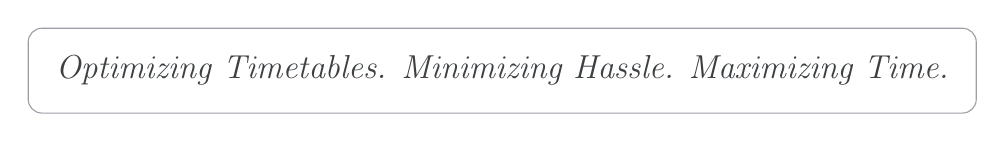
\begin{tikzpicture}
            \node[
                draw=mediumgray,
                rounded corners=5pt,
                inner sep=10pt,
                font=\large\itshape
            ] {\color{textdark}Optimizing Timetables. Minimizing Hassle. Maximizing Time.};
        \end{tikzpicture}
        
        \vspace{1.5cm}
        
        % Visual Icon
        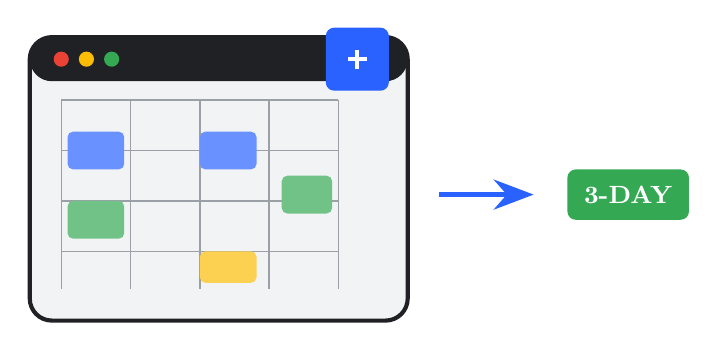
\begin{tikzpicture}[scale=0.8]
            % Browser window
            \draw[fill=lightgray, rounded corners=8pt, line width=1.5pt, draw=darkbg] 
                (-3, -2) rectangle (3, 2.5);
            \fill[darkbg, rounded corners=8pt] (-3, 1.8) rectangle (3, 2.5);
            
            % Browser dots
            \fill[dangerred] (-2.5, 2.15) circle (0.12);
            \fill[warningorange] (-2.1, 2.15) circle (0.12);
            \fill[accentgreen] (-1.7, 2.15) circle (0.12);
            
            % Extension icon
            \node[
                fill=primaryblue,
                rounded corners=3pt,
                minimum size=0.8cm
            ] at (2.2, 2.15) {};
            \draw[white, line width=1.5pt] (2.05, 2.15) -- (2.35, 2.15);
            \draw[white, line width=1.5pt] (2.2, 2.0) -- (2.2, 2.3);
            
            % Calendar grid
            \foreach \i in {0, 1, 2, 3, 4} {
                \draw[mediumgray, line width=0.5pt] (-2.5 + \i*1.1, 1.5) -- (-2.5 + \i*1.1, -1.5);
            }
            \foreach \i in {0, 1, 2, 3} {
                \draw[mediumgray, line width=0.5pt] (-2.5, 1.5 - \i*0.8) -- (1.9, 1.5 - \i*0.8);
            }
            
            % Sample course blocks
            \fill[primaryblue!70, rounded corners=2pt] (-2.4, 1.0) rectangle (-1.5, 0.4);
            \fill[accentgreen!70, rounded corners=2pt] (-2.4, -0.1) rectangle (-1.5, -0.7);
            \fill[primaryblue!70, rounded corners=2pt] (-0.3, 1.0) rectangle (0.6, 0.4);
            \fill[warningorange!70, rounded corners=2pt] (-0.3, -0.9) rectangle (0.6, -1.4);
            \fill[accentgreen!70, rounded corners=2pt] (1.0, 0.3) rectangle (1.8, -0.3);
            
            % Optimization arrow
            \draw[-{Stealth[scale=1.2]}, line width=2pt, primaryblue] 
                (3.5, 0) -- (5, 0);
            
            % Optimized indicator
            \node[
                fill=accentgreen,
                text=white,
                font=\small\bfseries,
                rounded corners=3pt,
                inner sep=6pt
            ] at (6.5, 0) {3-DAY};
        \end{tikzpicture}
        
        \vspace{2cm}
        
        % Team Members
        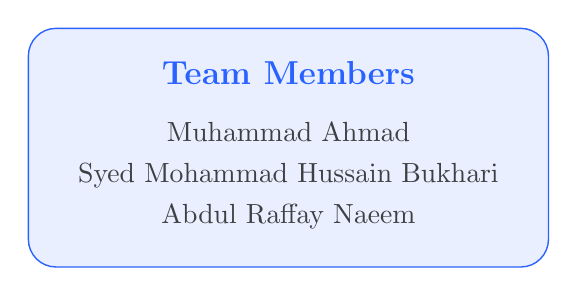
\begin{tikzpicture}
            \node[
                fill=primaryblue!10,
                rounded corners=10pt,
                inner sep=12pt,
                draw=primaryblue,
                line width=0.5pt
            ] {
                \begin{tabular}{c}
                    {\large\bfseries\color{primaryblue} Team Members}\\[0.3cm]
                    {\color{textdark} Muhammad Ahmad}\\[0.1cm]
                    {\color{textdark} Syed Mohammad Hussain Bukhari}\\[0.1cm]
                    {\color{textdark} Abdul Raffay Naeem}
                \end{tabular}
            };
        \end{tikzpicture}
        
        \vspace{0.8cm}
        
        % University Info
        
\begin{tikzpicture}
            \node[
                fill=boxbg,
                rounded corners=10pt,
                inner sep=15pt
            ] {
                \begin{tabular}{c}
                    {\Large\bfseries\color{ucpmaroon} University of Central Punjab}\\[0.3cm]
                    {\large\color{textdark} Faculty of Information Technology}\\[0.2cm]
                    {\color{mediumgray} January 2026}
                \end{tabular}
            };
        \end{tikzpicture}
    \end{center}
\end{titlepage}

%--------------------------------------------------------------
% TABLE OF CONTENTS
%--------------------------------------------------------------
\tableofcontents
\newpage

%--------------------------------------------------------------
% SECTION 1: PROBLEM IDENTIFICATION
%--------------------------------------------------------------
\section{Problem Identification}

\begin{questionbox}{What specific campus-life problem are you solving?}
The UCP Odoo-based course registration system requires students to \highlight{manually browse} through course sections, checking timings and availability \textbf{one-by-one} using an add-to-cart system. Students must mentally calculate:
\begin{itemize}[leftmargin=20pt, itemsep=2pt]
    \item[\faIcon{times-circle}] Schedule conflicts between sections
    \item[\faIcon{times-circle}] Gaps between consecutive classes
    \item[\faIcon{times-circle}] Optimal distribution across campus days
\end{itemize}
This tedious \textbf{trial-and-error} process consumes \highlight{30 to 60+ minutes} each semester.
\end{questionbox}

% Problem Visualization Diagram
\begin{center}
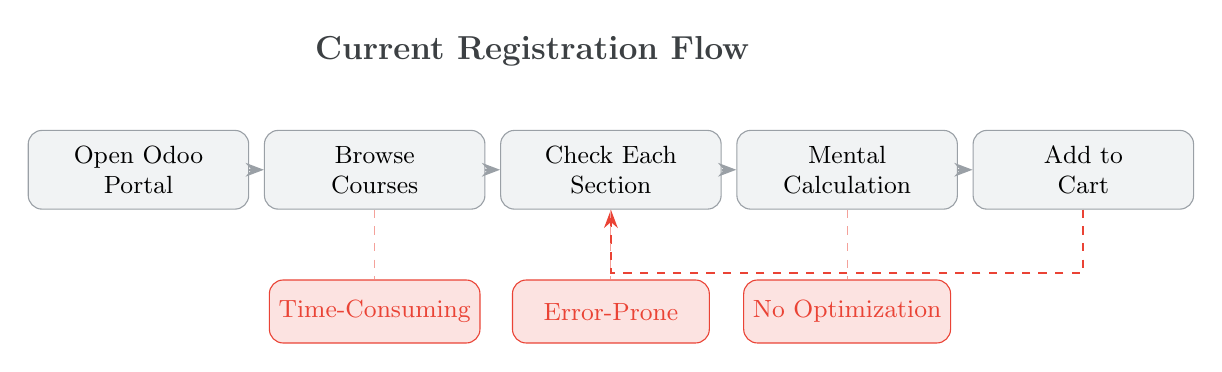
\begin{tikzpicture}[
    node distance=0.8cm,
    stepnode/.style={
        rectangle,
        rounded corners=5pt,
        draw=mediumgray,
        fill=lightgray,
        minimum width=2.8cm,
        minimum height=1cm,
        align=center,
        font=\small
    },
    painnode/.style={
        rectangle,
        rounded corners=5pt,
        fill=dangerred!15,
        draw=dangerred,
        minimum width=2.5cm,
        minimum height=0.8cm,
        align=center,
        font=\small\color{dangerred}
    },
    arr/.style={-{Stealth}, thick, color=mediumgray}
]
    % Title
    \node[font=\large\bfseries\color{textdark}] at (0, 3) {Current Registration Flow};
    
    % Steps
    \node[stepnode] (s1) at (-5, 1.5) {Open Odoo\\Portal};
    \node[stepnode] (s2) at (-2, 1.5) {Browse\\Courses};
    \node[stepnode] (s3) at (1, 1.5) {Check Each\\Section};
    \node[stepnode] (s4) at (4, 1.5) {Mental\\Calculation};
    \node[stepnode] (s5) at (7, 1.5) {Add to\\Cart};
    
    % Arrows
    \draw[arr] (s1) -- (s2);
    \draw[arr] (s2) -- (s3);
    \draw[arr] (s3) -- (s4);
    \draw[arr] (s4) -- (s5);
    
    % Loop back arrow
    \draw[arr, dangerred, dashed] (s5.south) -- ++(0, -0.8) -| node[pos=0.25, below, font=\small\color{dangerred}]{Conflict Found!} (s3.south);
    
    % Pain points
    \node[painnode] (p1) at (-2, -0.3) {Time-Consuming};
    \node[painnode] (p2) at (1, -0.3) {Error-Prone};
    \node[painnode] (p3) at (4, -0.3) {No Optimization};
    
    \draw[dashed, dangerred!50] (s2.south) -- (p1.north);
    \draw[dashed, dangerred!50] (s3.south) -- (p2.north);
    \draw[dashed, dangerred!50] (s4.south) -- (p3.north);
\end{tikzpicture}
\end{center}

\vspace{0.5cm}

\begin{questionbox}{Who is most affected by this problem?}
\begin{center}
\begin{tikzpicture}[
    userbox/.style={
        rectangle,
        rounded corners=8pt,
        fill=primaryblue!10,
        draw=primaryblue,
        minimum width=3.5cm,
        minimum height=1.8cm,
        align=center
    }
]
    \node[userbox] (u1) at (0, 0) {\faIcon{users}\\[3pt]\textbf{16,000+}\\Students};
    \node[userbox] (u2) at (4.5, 0) {\faIcon{bus}\\[3pt]\textbf{Commuters}\\(Majority)};
    \node[userbox] (u3) at (9, 0) {\faIcon{clock}\\[3pt]\textbf{Peak Hour}\\Registrants};
    
    \draw[-{Stealth}, thick, primaryblue] (u1) -- (u2);
    \draw[-{Stealth}, thick, primaryblue] (u2) -- (u3);
\end{tikzpicture}
\end{center}
\end{questionbox}

\begin{questionbox}{How often does this problem occur?}
\begin{center}
\stat{2$\times$}{per year (each semester)} \hspace{1cm}
\stat{32,000}{registration sessions annually}
\end{center}
Additional stress during \textbf{add/drop weeks} when sections rapidly open and close.
\end{questionbox}

\begin{questionbox}{How is this problem currently addressed, and why is it inadequate?}
\vspace{0.3cm}
\begin{center}
\begin{tikzpicture}[
    method/.style={
        rectangle,
        rounded corners=5pt,
        fill=warningorange!15,
        draw=warningorange,
        minimum width=3cm,
        minimum height=1.2cm,
        align=center,
        font=\small
    },
    issue/.style={
        rectangle,
        rounded corners=3pt,
        fill=dangerred!10,
        font=\scriptsize\color{dangerred},
        inner sep=4pt
    }
]
    \node[method] (m1) at (0, 0) {\faIcon{folder-open}\\Manual Browsing};
    \node[method] (m2) at (4, 0) {\faIcon{table}\\External\\Spreadsheets};
    \node[method] (m3) at (8, 0) {\faIcon{redo}\\Trial \& Error\\in Cart};
    \node[method] (m4) at (12, 0) {\faIcon{sync}\\Constant\\Refreshing};
    
    \node[issue, below=0.4cm of m1] {Slow \& tedious};
    \node[issue, below=0.4cm of m2] {Context switching};
    \node[issue, below=0.4cm of m3] {No optimization};
    \node[issue, below=0.4cm of m4] {Sections close};
\end{tikzpicture}
\end{center}
\end{questionbox}

%--------------------------------------------------------------
% SECTION 2: IMPACT & RELEVANCE
%--------------------------------------------------------------
\newpage
\section{Impact \& Relevance}

\begin{questionbox}{What negative impact does this problem have on students?}
\end{questionbox}

\begin{impactbox}
\begin{center}
\begin{tikzpicture}[
    impact/.style={
        circle,
        fill=dangerred!20,
        draw=dangerred,
        minimum size=2.2cm,
        align=center,
        font=\small
    }
]
    \node[impact] (i1) at (0, 0) {\faIcon{hourglass-half}\\[3pt]\textbf{30--60 min}\\wasted};
    \node[impact] (i2) at (3.5, 0) {\faIcon{calendar-times}\\[3pt]\textbf{5-day}\\schedules};
    \node[impact] (i3) at (7, 0) {\faIcon{exclamation-triangle}\\[3pt]\textbf{Anxiety}\\\& stress};
    \node[impact] (i4) at (10.5, 0) {\faIcon{car}\\[3pt]\textbf{Extra}\\commute};
    \node[impact] (i5) at (14, 0) {\faIcon{battery-quarter}\\[3pt]\textbf{Large}\\gaps};
    
    % Labels below
    \node[font=\scriptsize, text=textdark] at (0, -1.6) {Time Waste};
    \node[font=\scriptsize, text=textdark] at (3.5, -1.6) {Poor Schedules};
    \node[font=\scriptsize, text=textdark] at (7, -1.6) {Reg. Anxiety};
    \node[font=\scriptsize, text=textdark] at (10.5, -1.6) {Physical Toll};
    \node[font=\scriptsize, text=textdark] at (14, -1.6) {Wasted Time};
\end{tikzpicture}
\end{center}
\end{impactbox}

\vspace{0.5cm}

\begin{questionbox}{How many students are likely affected?}
\end{questionbox}

\begin{center}
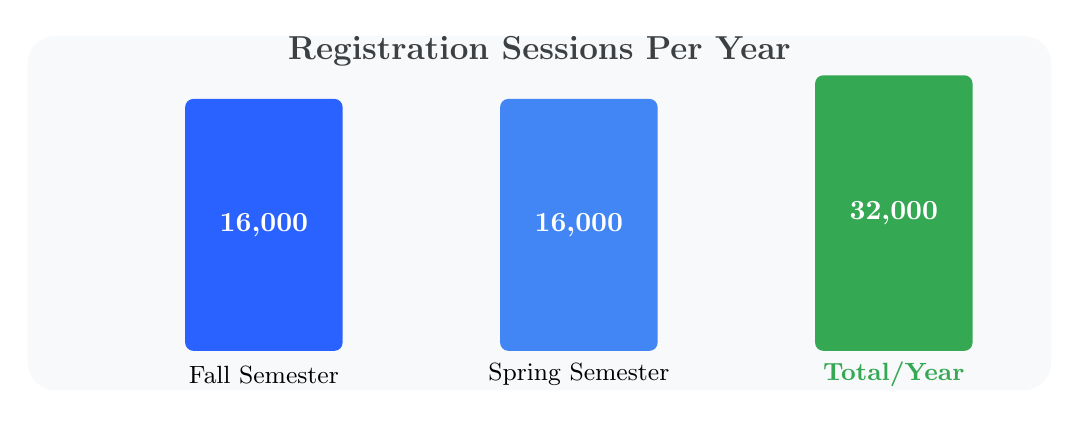
\begin{tikzpicture}
    % Bar chart background
    \fill[boxbg, rounded corners=10pt] (-1, -0.5) rectangle (12, 4);
    
    % Bars
    \fill[primaryblue, rounded corners=3pt] (1, 0) rectangle (3, 3.2);
    \fill[secondaryblue, rounded corners=3pt] (5, 0) rectangle (7, 3.2);
    \fill[accentgreen, rounded corners=3pt] (9, 0) rectangle (11, 3.5);
    
    % Labels
    \node[font=\bfseries\color{white}] at (2, 1.6) {16,000};
    \node[font=\bfseries\color{white}] at (6, 1.6) {16,000};
    \node[font=\bfseries\color{white}] at (10, 1.75) {32,000};
    
    % Bottom labels
    \node[font=\small] at (2, -0.3) {Fall Semester};
    \node[font=\small] at (6, -0.3) {Spring Semester};
    \node[font=\small\bfseries, color=accentgreen] at (10, -0.3) {Total/Year};
    
    % Title
    \node[font=\large\bfseries, color=textdark] at (5.5, 3.8) {Registration Sessions Per Year};
\end{tikzpicture}
\end{center}

%--------------------------------------------------------------
% SECTION 3: SOLUTION CONCEPT
%--------------------------------------------------------------
\newpage
\section{Solution Concept}

\begin{questionbox}{Briefly describe your proposed solution}
A \highlight{Chrome Extension} that integrates directly with the UCP Odoo portal to automatically extract course data, generate optimized timetables, and enable one-click registration.
\end{questionbox}

\begin{solutionbox}
\begin{center}
\begin{tikzpicture}[
    node distance=1.5cm,
    block/.style={
        rectangle,
        rounded corners=8pt,
        draw=primaryblue,
        fill=primaryblue!10,
        minimum width=3.5cm,
        minimum height=1.5cm,
        align=center,
        font=\small
    },
    arr/.style={-{Stealth[scale=1.2]}, thick, primaryblue}
]
    % Title
    \node[font=\Large\bfseries\color{accentgreen}] at (5, 4.5) {Solution Architecture};
    
    % Blocks
    \node[block] (ext) at (0, 2.5) {\faIcon{puzzle-piece}\\Chrome Extension};
    \node[block] (odoo) at (0, 0) {\faIcon{globe}\\Odoo Portal};
    \node[block] (extract) at (4, 2.5) {\faIcon{database}\\Data Extraction};
    \node[block] (input) at (4, 0) {\faIcon{sliders-h}\\User Preferences};
    \node[block] (algo) at (8, 1.25) {\faIcon{cogs}\\Optimization\\Algorithm};
    \node[block] (output) at (12, 1.25) {\faIcon{calendar-check}\\Optimized\\Timetable};
    
    % Arrows
    \draw[arr] (odoo) -- (ext);
    \draw[arr] (ext) -- (extract);
    \draw[arr] (input) -- (algo);
    \draw[arr] (extract) -- (algo);
    \draw[arr] (algo) -- (output);
    
    % Data flow labels
    \node[font=\tiny, color=mediumgray] at (2, 2.8) {Scrapes data};
    \node[font=\tiny, color=mediumgray] at (6.2, 2.2) {Course sections};
    \node[font=\tiny, color=mediumgray] at (6.2, 0.3) {Days, gaps, times};
    \node[font=\tiny, color=mediumgray] at (10, 1.6) {Ranked options};
\end{tikzpicture}
\end{center}
\end{solutionbox}

\vspace{0.5cm}

\subsection{Core MVP Features}

\begin{center}
\begin{tikzpicture}[
    feature/.style={
        rectangle,
        rounded corners=10pt,
        fill=white,
        draw=secondaryblue,
        line width=1pt,
        minimum width=6.5cm,
        minimum height=1.6cm,
        align=left,
        font=\small,
        drop shadow={opacity=0.1}
    }
]
    % Features
    \node[feature] (f1) at (0, 3) {
        \textcolor{primaryblue}{\faIcon{search}} \textbf{Data Extraction}\\
        \hspace{0.5cm}Auto-scrape course sections from Odoo
    };
    
    \node[feature] (f2) at (8, 3) {
        \textcolor{primaryblue}{\faIcon{edit}} \textbf{Preference Input}\\
        \hspace{0.5cm}Days, gaps, time slots
    };
    
    \node[feature] (f3) at (0, 0.8) {
        \textcolor{accentgreen}{\faIcon{magic}} \textbf{Optimization Engine}\\
        \hspace{0.5cm}Generate \& rank best timetables
    };
    
    \node[feature] (f4) at (8, 0.8) {
        \textcolor{accentgreen}{\faIcon{eye}} \textbf{Visual Display}\\
        \hspace{0.5cm}Color-coded weekly calendar
    };
    
    \node[feature] (f5) at (4, -1.4) {
        \textcolor{warningorange}{\faIcon{bolt}} \textbf{Quick Registration}\\
        \hspace{0.5cm}One-click cart auto-fill (Stretch)
    };
    
    % Connecting lines
    \draw[dashed, mediumgray] (f1) -- (f2);
    \draw[dashed, mediumgray] (f1) -- (f3);
    \draw[dashed, mediumgray] (f2) -- (f4);
    \draw[dashed, mediumgray] (f3) -- (f5);
    \draw[dashed, mediumgray] (f4) -- (f5);
\end{tikzpicture}
\end{center}

\subsection{How does your solution improve the daily campus experience?}

\begin{center}
\begin{tikzpicture}[
    before/.style={
        rectangle,
        rounded corners=5pt,
        fill=dangerred!15,
        draw=dangerred,
        minimum width=4cm,
        minimum height=1cm,
        align=center
    },
    after/.style={
        rectangle,
        rounded corners=5pt,
        fill=accentgreen!15,
        draw=accentgreen,
        minimum width=4cm,
        minimum height=1cm,
        align=center
    }
]
    % Headers
    \node[font=\bfseries\color{dangerred}] at (-3, 3) {\faIcon{times-circle} BEFORE};
    \node[font=\bfseries\color{accentgreen}] at (3, 3) {\faIcon{check-circle} AFTER};
    
    % Comparison items
    \node[before] at (-3, 2) {45+ minutes};
    \node[after] at (3, 2) {\textbf{Under 5 min}};
    \draw[-{Stealth}, thick, primaryblue] (-0.5, 2) -- (0.5, 2);
    
    \node[before] at (-3, 0.8) {5-day schedule};
    \node[after] at (3, 0.8) {\textbf{3-day schedule}};
    \draw[-{Stealth}, thick, primaryblue] (-0.5, 0.8) -- (0.5, 0.8);
    
    \node[before] at (-3, -0.4) {Large gaps};
    \node[after] at (3, -0.4) {\textbf{Minimal gaps}};
    \draw[-{Stealth}, thick, primaryblue] (-0.5, -0.4) -- (0.5, -0.4);
    
    \node[before] at (-3, -1.6) {High stress};
    \node[after] at (3, -1.6) {\textbf{Zero stress}};
    \draw[-{Stealth}, thick, primaryblue] (-0.5, -1.6) -- (0.5, -1.6);
\end{tikzpicture}
\end{center}

%--------------------------------------------------------------
% SECTION 4: USERS & VALIDATION
%--------------------------------------------------------------
\newpage
\section{Users \& Validation}

\begin{questionbox}{Who is your primary user?}
\end{questionbox}

\begin{center}
\begin{tikzpicture}[
    persona/.style={
        rectangle,
        rounded corners=12pt,
        fill=boxbg,
        draw=primaryblue,
        line width=1.5pt,
        minimum width=4.5cm,
        minimum height=3.5cm,
        align=center
    }
]
    % Personas
    \node[persona] (p1) at (0, 0) {
        \textcolor{primaryblue}{\faIcon[regular]{user-circle}}\\[5pt]
        \textbf{Commuter Students}\\[3pt]
        {\small Want fewer}\\
        {\small campus days}
    };
    
    \node[persona] (p2) at (5.5, 0) {
        \textcolor{accentgreen}{\faIcon{user-clock}}\\[5pt]
        \textbf{Time-Conscious}\\[3pt]
        {\small Need efficient}\\
        {\small schedules}
    };
    
    \node[persona] (p3) at (11, 0) {
        \textcolor{warningorange}{\faIcon{user-graduate}}\\[5pt]
        \textbf{All UCP Students}\\[3pt]
        {\small Frustrated with}\\
        {\small current system}
    };
    
    % Priority indicators
    \node[fill=dangerred, text=white, font=\tiny\bfseries, rounded corners=2pt, inner sep=3pt] at (0, 2) {HIGH PRIORITY};
    \node[fill=warningorange, text=white, font=\tiny\bfseries, rounded corners=2pt, inner sep=3pt] at (5.5, 2) {PRIORITY};
    \node[fill=primaryblue, text=white, font=\tiny\bfseries, rounded corners=2pt, inner sep=3pt] at (11, 2) {ALL USERS};
\end{tikzpicture}
\end{center}

\vspace{1cm}

\begin{questionbox}{How will you validate that they need your solution?}
\end{questionbox}

\subsection{Phase 1 Validation (Today)}

\begin{center}
\begin{tikzpicture}[
    method/.style={
        rectangle,
        rounded corners=8pt,
        fill=primaryblue!10,
        draw=primaryblue,
        minimum width=5.5cm,
        minimum height=2cm,
        align=center
    }
]
    \node[method] (m1) at (0, 0) {
        \faIcon{comments}\\[5pt]
        \textbf{Quick Hallway Surveys}\\
        {\small "How long does registration take?"}
    };
    
    \node[method] (m2) at (7, 0) {
        \faIcon{user-friends}\\[5pt]
        \textbf{Student Interviews}\\
        {\small 8--10 students about experiences}
    };
    
    \node[method] (m3) at (3.5, -3) {
        \faIcon{poll}\\[5pt]
        \textbf{Preference Poll}\\
        {\small 3 packed days vs 5 spread days?}
    };
\end{tikzpicture}
\end{center}

\subsection{Phase 2 Validation (Planned)}

\begin{center}
\begin{tabular}{>{\columncolor{primaryblue!10}}c p{8cm}}
    \toprule
    \textbf{Method} & \textbf{Description} \\
    \midrule
    \faIcon{palette} & Show mockups/wireframes of extension UI \\
    \faIcon{laptop-code} & Demonstrate working prototype to 15--20 students \\
    \faIcon{clipboard-list} & Observe reactions and gather feature requests \\
    \faIcon{chart-bar} & Validate optimization preferences \\
    \bottomrule
\end{tabular}
\end{center}

\subsection{Validation Questions}

\begin{enumerate}[leftmargin=25pt]
    \item[\faIcon{question-circle}] ``How long does course registration typically take you?''
    \item[\faIcon{question-circle}] ``What's the most frustrating part of registration?''
    \item[\faIcon{question-circle}] ``Do you prefer fewer days with packed schedule OR more days with gaps?''
    \item[\faIcon{question-circle}] ``Have you ever ended up with a schedule you weren't happy with?''
    \item[\faIcon{question-circle}] ``Would you use a Chrome extension that auto-generates optimal timetables?''
\end{enumerate}

%--------------------------------------------------------------
% SECTION 5: TECHNICAL APPROACH
%--------------------------------------------------------------
\newpage
\section{Technical Approach}

\subsection{Technology Stack}

\begin{center}
\begin{tikzpicture}[
    tech/.style={
        rectangle,
        rounded corners=8pt,
        fill=darkbg,
        text=white,
        minimum width=3.2cm,
        minimum height=1.4cm,
        align=center,
        font=\small
    },
    label/.style={
        font=\footnotesize\color{mediumgray}
    }
]
    % Stack layers
    \node[tech] (t1) at (0, 0) {\faIcon{html5} HTML/CSS/JS\\Chrome APIs};
    \node[tech] (t2) at (4.5, 0) {\faIcon{file-code} Content Script\\DOM Scraping};
    \node[tech] (t3) at (9, 0) {\faIcon{cog} Background\\Script};
    \node[tech] (t4) at (13.5, 0) {\faIcon{database} Local Storage};
    
    % Labels
    \node[label] at (0, -1.1) {Frontend};
    \node[label] at (4.5, -1.1) {Data Layer};
    \node[label] at (9, -1.1) {Logic Layer};
    \node[label] at (13.5, -1.1) {Persistence};
    
    % Connections
    \draw[-{Stealth}, thick, secondaryblue] (t1) -- (t2);
    \draw[-{Stealth}, thick, secondaryblue] (t2) -- (t3);
    \draw[-{Stealth}, thick, secondaryblue] (t3) -- (t4);
\end{tikzpicture}
\end{center}

\subsection{Development Timeline}

\begin{center}
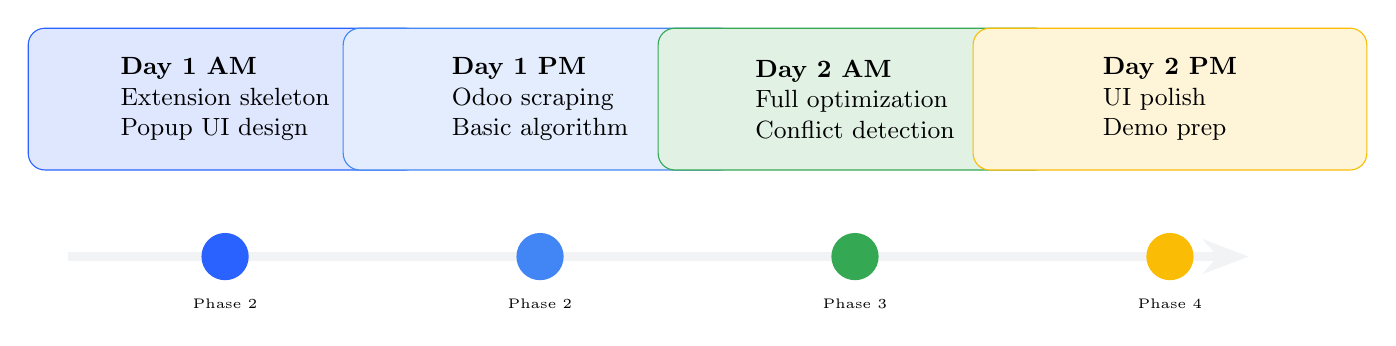
\begin{tikzpicture}[
    phase/.style={
        rectangle,
        rounded corners=6pt,
        minimum width=5cm,
        minimum height=1.8cm,
        align=left,
        font=\small
    }
]
    % Timeline arrow
    \draw[-{Stealth}, line width=3pt, lightgray] (-1, 0) -- (14, 0);
    
    % Phase markers
    \fill[primaryblue] (1, 0) circle (0.3);
    \fill[secondaryblue] (5, 0) circle (0.3);
    \fill[accentgreen] (9, 0) circle (0.3);
    \fill[warningorange] (13, 0) circle (0.3);
    
    % Phase labels
    \node[phase, fill=primaryblue!15, draw=primaryblue] at (1, 2) {
        \textbf{Day 1 AM}\\
        Extension skeleton\\
        Popup UI design
    };
    
    \node[phase, fill=secondaryblue!15, draw=secondaryblue] at (5, 2) {
        \textbf{Day 1 PM}\\
        Odoo scraping\\
        Basic algorithm
    };
    
    \node[phase, fill=accentgreen!15, draw=accentgreen] at (9, 2) {
        \textbf{Day 2 AM}\\
        Full optimization\\
        Conflict detection
    };
    
    \node[phase, fill=warningorange!15, draw=warningorange] at (13, 2) {
        \textbf{Day 2 PM}\\
        UI polish\\
        Demo prep
    };
    
    % Time labels
    \node[font=\tiny] at (1, -0.6) {Phase 2};
    \node[font=\tiny] at (5, -0.6) {Phase 2};
    \node[font=\tiny] at (9, -0.6) {Phase 3};
    \node[font=\tiny] at (13, -0.6) {Phase 4};
\end{tikzpicture}
\end{center}

%--------------------------------------------------------------
% SECTION 6: EXPECTED OUTPUT
%--------------------------------------------------------------
\section{Expected Output Summary}

\begin{center}
\begin{tikzpicture}[
    check/.style={
        rectangle,
        rounded corners=8pt,
        fill=accentgreen!10,
        draw=accentgreen,
        line width=1pt,
        minimum width=13cm,
        minimum height=1.2cm,
        align=left,
        font=\normalsize
    }
]
    \node[check] at (0, 3) {\textcolor{accentgreen}{\faIcon{check-circle}} \textbf{Clear Problem Interpretation}: Students waste time manually building schedules in Odoo};
    
    \node[check] at (0, 1.5) {\textcolor{accentgreen}{\faIcon{check-circle}} \textbf{Identified Target Users}: All 16,000+ UCP students, especially daily commuters};
    
    \node[check] at (0, 0) {\textcolor{accentgreen}{\faIcon{check-circle}} \textbf{Solution Approach}: Chrome extension integrated directly with Odoo portal};
    
    \node[check] at (0, -1.5) {\textcolor{accentgreen}{\faIcon{check-circle}} \textbf{High-Level MVP}: Auto-generate and rank optimized timetables based on preferences};
\end{tikzpicture}
\end{center}

\vspace{1cm}

\begin{center}

\begin{tikzpicture}
    \node[
        rectangle,
        rounded corners=15pt,
        fill=ucpmaroon,
        text=white,
        minimum width=12cm,
        minimum height=2.5cm,
        align=center,
        font=\Large,
        drop shadow
    ] {
        \faIcon{rocket} \textbf{Ready for Phase 2: User Research \& Validation}\\[8pt]
        {\normalsize Building a solution that saves 40+ minutes per student, per semester}
    };
\end{tikzpicture}
\end{center}

%--------------------------------------------------------------
% END DOCUMENT
%--------------------------------------------------------------
\end{document}
